% !TEX root = main.tex

\section{Lecture 13: More GVCs: Dia-surface transport}
\begin{flushright}\textbf{[by Eva Cougnon]}\end{flushright}

In this lecture, we develop the concept of dia-surface transport. We can look at it as being a transfer of momentum or tracer across a surface. In previous lectures, we discussed about General Vertical Coordinates (GCVs) and kinematic boundary conditions (lectures~\ref{sec:lecture8} and~\ref{sec:lecture10}), some of what is shown here is based on these two lectures. The goal here is to express the material time derivative operator using GCVs.

\subsection{Flow normal to the surface}
The diagram below illustrates a surface $\sigma$ which is function of space and time, $x, y, z$ and $t$. 
\begin{figure}[h!]
\centering
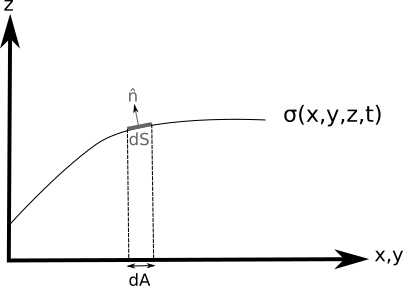
\includegraphics[width=0.4\textwidth]{figures/lecture13_fig1_GVC.png}
\caption{Schematic view of a  dia-surface transport across a surface $\sigma$. The direction normal for a surface element $\mathrm{d}S$ along $\sigma$ is noted $\boldsymbol{\hat{n}}$. The horizontal projection of the surface element $\mathrm{d}S$ is denoted as $\mathrm{d}A = |cos \theta| \mathrm{d}S$, where $\theta$ is the angle between the surface and the horizontal. The vertical stratification should remain non-zero ($\partial_z\sigma\ne0$), the surface element cannot be vertical, so we can relate $\mathrm{d}S$ and $\mathrm{d}A$.
%{\color{red}and should always be different from zero, which means that the surface element cannot be vertical ($\partial \sigma / \partial z \neq 0$). [Navid: The red part here by itself doesn't make sense. The condition $\partial_z\sigma\ne0$ should hold only if we want to relate $dS$ and $dA$.]}
}
\label{schem1}
\end{figure}

By definition, the flux of matter crossing the surface element in the direction normal is equal to:
\begin{equation}
\centering
\text{flux  in  direction } \hat{\boldsymbol{n}} = \boldsymbol{v} \cdot \hat{\boldsymbol{n}},
\label{normal}
\end{equation}
where $\boldsymbol{v}$ is the vector velocity of the fluid particle and where the surface unit normal is:
\begin{equation}
\centering
\hat{\boldsymbol{n}} = \frac{\boldsymbol{\nabla} \sigma}{|\boldsymbol{\nabla} \sigma|}. \label{eq13.2}
\end{equation}

When we take into account that the $\sigma$ surface may move in time, as it is usually the case, the flux of matter across the surface is:
\begin{equation}
\centering
\text{flux of matter crossing surface} = \hat{\boldsymbol{n}} \cdot (\boldsymbol{v}-\boldsymbol{v}^{(\sigma)}),
\end{equation}
where with $\boldsymbol{v}^{(\sigma)}$ we denote the velocity of the surface $\sigma$. The velocity of a point on the surface element satisfies:
\begin{equation}
\frac{\partial \sigma}{\partial t} + \boldsymbol{v}^{(\sigma)} \cdot \boldsymbol{\nabla} \sigma = 0,
\label{partialtimederiv}
\end{equation}
and the material time derivative being:
\begin{equation}
\frac{\mathrm{D}\sigma}{\mathrm{D}t} = \frac{\partial \sigma}{\partial t} + \boldsymbol{v} \cdot \boldsymbol{\nabla} \sigma,
\label{mattimederiv}
\end{equation}
we can estimate the flux of matter crossing the surface by rearranging equations \eqref{partialtimederiv} and \eqref{mattimederiv}:
\begin{equation}
\frac{\mathrm{D}\sigma}{\mathrm{D}t} = - \boldsymbol{v}^{(\sigma)} \cdot \boldsymbol{\nabla} \sigma + \boldsymbol{v} \cdot \boldsymbol{\nabla} \sigma.
\end{equation}

Using equation \eqref{eq13.2} we get:
\begin{equation}
\frac{\mathrm{D}\sigma}{\mathrm{D}t} = \quad |\boldsymbol{\nabla} \sigma|\hat{\boldsymbol{n}} \cdot (\boldsymbol{v}-\boldsymbol{v}^{(\sigma)}),
\end{equation}
and finally the flux of matter across the surface is:
\begin{equation}
\hat{\boldsymbol{n}} \cdot (\boldsymbol{v}-\boldsymbol{v}^{(\sigma)}) = \frac{1}{|\boldsymbol{\nabla} \sigma|} \underbrace{\frac{\mathrm{D} \sigma}{\mathrm{D}t}}_{\equiv \dot{\sigma}}.
\label{fluxacrosssurf}
\end{equation}
where we introduce shorthand $\dot{\sigma}=\mathrm{D}\sigma/\mathrm{D} t$.

This is the net flux of fluid crossing the GVC surface. If no fluid crosses the surface, then the the material time derivative of the GVC surface, $\mathrm{D}\sigma/\mathrm{D}t$, vanishes and vice versa. This results is important in geophysical fluid mechanics and is seen in oceanography in isopycnal models and subduction calculations.


\subsection{Dia-surface transport and its velocity component}

We can use the area of the surface $\mathrm{d}S$ to normalised the volume flux in equation \eqref{fluxacrosssurf}. $\mathrm{d}S$ is an infinitesimal patch on the surface of constant GVC, $\sigma$, with outward unit normal $\boldsymbol{\hat{n}}$, as presented in Figure~\ref{schem1}. $\mathrm{d}A$ is the horizontal projection of this area. Then, the transport of fluid crossing the surface is
\begin{equation}
\frac{\dot{\sigma}}{|\boldsymbol{\nabla} \sigma|} \mathrm{d}S .
\end{equation}

Following rules of trigonometry introduced in lecture~\ref{sec:lecture8} (``Dynamic and permeable surface'') we can express the area factor,  $\mathrm{d}S/|\boldsymbol{\nabla} \sigma|$, as a function of $\mathrm{d}A$. To do so, we need to assume that the values of $\sigma$ depend monotonically with $z$. In that case we introduce the angle $\theta$ between the surface and the horizontal plane. Therefore, $\mathrm{d}A=|\cos \theta| \; \mathrm{d}S$ and the area factor is:
\begin{align} 
\frac{\mathrm{d}S}{|\boldsymbol{\nabla} \sigma|} & = \frac{\mathrm{d}S}{\sqrt{\big(\frac{\partial \sigma}{\partial x}\big)^2+\big(\frac{\partial \sigma}{\partial y}\big)^2+\big(\frac{\partial \sigma}{\partial z}\big)^2}} \nonumber\\
& = \frac{\mathrm{d}S}{\big|\frac{\partial \sigma}{\partial z}\big| \sqrt{ \left(\tfrac{\partial \sigma/\partial x}{\partial \sigma/\partial z}\right)^2 + \left(\tfrac{\partial \sigma/\partial y}{\partial \sigma/\partial z}\right)^2 +1}} \nonumber\\
& = \frac{\mathrm{d}S}{\big|\frac{\partial \sigma}{\partial z}\big| \sqrt{ \left(\frac{\partial z}{\partial x}\right)^2 + \left(\frac{\partial z}{\partial y}\right)^2 +1}} \nonumber\qquad\text{(but }(\tfrac{\partial z}{\partial x})^2 + (\tfrac{\partial z}{\partial y})^2 = \tan^2\theta\text{)} \\
% }_\text{squared slope of surface = $\tan^2\theta$}
& = \frac{\mathrm{d}S}{\big|\frac{\partial \sigma}{\partial z}\big| \sqrt{1 + \tan^2 \theta}} \nonumber\\
& = \biggr\rvert\frac{\partial z}{\partial \sigma}\biggr\lvert \; |\cos \theta| \; \mathrm{d}S \nonumber\\
& = \underbrace{\biggr\rvert\frac{\partial z}{\partial \sigma}\biggr\lvert}_\text{specific thickness} \; \mathrm{d}A.  \label{eq13.10}
\end{align}

Equation~\eqref{eq13.10} allows us to define the dia-surface velocity component for the GVC coordinate system, $w^{(\dot{\sigma})}$, which corresponds to the volume of fluid passing through the surface per unit horizontal area, per unit time:
\begin{equation}
\begin{aligned}
w^{(\dot{\sigma})} & = \hat{\boldsymbol{n}} \cdot (\boldsymbol{v}-\boldsymbol{v}^{(\sigma)}) \frac{\mathrm{d}S}{\mathrm{d}A} \\
& = \frac{(\text{volume}/\text{time}) \: of fluid through surface}{\text{horizontal area of surface}} \\
& = \frac{\partial z}{\partial \sigma} \dot{\sigma}.
\end{aligned}
\label{VelComp1}
\end{equation}
This is a transport with units of velocity and $\partial z/\partial \sigma$ is the specific thickness. An alternative expression that comes from expanding the material time derivative from equation \eqref{fluxacrosssurf}, $\dot{\sigma} = \mathrm{D}\sigma/\mathrm{D}t = |\boldsymbol{\nabla} \sigma| \boldsymbol{\hat{n}} \cdot (\boldsymbol{v} - \boldsymbol{v}^\sigma)$ is:
\begin{align}
w^{(\dot{\sigma})} & =\frac{\partial z}{\partial \sigma} \dot{\sigma} \nonumber\\
& = \frac{\partial z}{\partial \sigma} \bigg (\frac{\partial \sigma}{\partial t} + \boldsymbol{v} \cdot \boldsymbol{\nabla} \sigma \bigg )
\label{wsigma}
\end{align}
By using the equations described above (equation \ref{wsigma}) and partial derivative operators (see \citet[Chapter 18.3 and 8.2 in][]{Griffies2019} for recall on partial derivative operators), we obtain the following equation:
\begin{equation}
w^{(\dot{\sigma})} = w - \bigg [\!\!\!\!\!\underbrace{\bigg (\frac{\partial}{\partial t}\bigg )_\sigma + \boldsymbol{u} \cdot \boldsymbol{\nabla}_\sigma}_{\substack{\text{horizontal material derivative}\\\text{on a surface of constant $\sigma$}}} \!\!\!\!\!\bigg ]z,
\label{VelComp}
\end{equation}
where $(\partial/\partial t)_\sigma$ is the time derivative along the $\sigma$ surface, and $\boldsymbol{\nabla}_\sigma z$ is the slope of the surface.
%[Navid: $(\boldsymbol{u} \cdot \boldsymbol{\nabla}_\sigma)z$ is not dimensionless as a slope should be. Did you meant to write ``$\boldsymbol{\nabla}_\sigma z$ is the slope''?]}.

Equation~\eqref{VelComp} relates the vertical component of the fluid particle velocity $w$ to the dia-surface velocity component $w^{(\dot{\sigma})}$. Therefore, when the GVC surface is static ($\partial z/\partial t$) the dia-surface velocity component described with equation \eqref{VelComp} becomes:
\begin{equation}
w^{(\dot{\sigma})} = w - \boldsymbol{u} \cdot \boldsymbol{\nabla}_\sigma z, \quad \text{for a static surface}.
\end{equation}
On the other hand, when the GVC the surface is flat, the dia-surface velocity components only represent the flux of fluid moving vertically relative to the motion of the GVC surface. But if the surface is both, flat and static (e.g., a constant geopotential), the dia-surface velocity component becomes the vertical velocity component only:
\begin{equation}
w^{(\dot{\sigma})} = w = \frac{\mathrm{D}z}{\mathrm{D}t}, \quad \text{for a static and flat surface}.
\end{equation}

\subsection{Material time-derivative in GVCs}

With the expression of the dia-surface velocity component for the GVC system, $w^{(\dot{\sigma})}$, equation~\eqref{VelComp1}, we can express the material time-derivative in three different ways which turn out to be useful in GVCs:
\begin{equation}
\begin{aligned}
\left(\frac{\mathrm{D}}{\mathrm{D}t}\right)_z & = \bigg (\frac{\partial}{\partial t} \bigg )_z + \underbrace{\boldsymbol{u} \cdot \boldsymbol{\nabla}_z}_{\substack{\text{horizontal}\\\text{gradient}}} \;\; +\!\!\!\! \underbrace{w\frac{\partial}{\partial z}}_{\substack{\text{gradient of}\\\text{vertical velocity}}} \\
\substack{\text{changing from Cartesian}\\\text{coordinates to GVCs:}}& =  \bigg (\frac{\partial}{\partial t} \bigg )_\sigma + \boldsymbol{u} \cdot \boldsymbol{\nabla}_\sigma + \underbrace{w^{(\dot{\sigma})}\frac{\partial}{\partial z}}_{\substack{\text{non-zero  transport}\\\text{across the surface}}} \\
& =  \bigg (\frac{\partial}{\partial t} \bigg )_\sigma + \boldsymbol{u} \cdot \boldsymbol{\nabla}_\sigma + \dot{\sigma}\frac{\partial}{\partial \sigma}.
\end{aligned}
\end{equation}
The relationship between  the two vertical coordinate partial derivative comes from the chain rule:
\begin{equation}
\frac{\partial}{\partial \sigma} = \frac{\partial z}{\partial \sigma} \frac{\partial}{\partial z}.
\end{equation}

\subsection{Velocity vector and fluid particle trajectories}

The velocity vector in Cartesian coordinates is:
\begin{equation}
\boldsymbol{v} = \boldsymbol{\hat{x}}u + \boldsymbol{\hat{y}}v + \boldsymbol{\hat{z}}w,
\end{equation}
and using $w$ from equation~\eqref{VelComp} we get:
\begin{equation}
\boldsymbol{v} =  \boldsymbol{\hat{x}}u + \boldsymbol{\hat{y}}v + \boldsymbol{\hat{z}} \bigg [w^{(\dot{\sigma})} + \bigg (\frac{\partial z}{\partial t} \bigg )_\sigma + \boldsymbol{u} \cdot\boldsymbol{\nabla}_\sigma z \bigg].
\end{equation}
By re-arranging and combining the $u$ terms we get:
\begin{align}
\boldsymbol{v} &=  u\underbrace{\bigg [\boldsymbol{\hat{x}} + \boldsymbol{\hat{z}}  \bigg (\!\overbrace{\frac{\partial z}{\partial x}}^{\substack{\text{slope}\\\text{term}}} \! \bigg )_\sigma \bigg]}_{=\boldsymbol{e}_{\bar{1}}} 
+ v  \underbrace{\bigg [\boldsymbol{\hat{y}} + \boldsymbol{\hat{z}}  \bigg (\!\overbrace{\frac{\partial z}{\partial y}}^{\substack{\text{slope}\\\text{term}}} \!\bigg )_\sigma \bigg]}_{=\boldsymbol{e}_{\bar{2}}} 
+ \bigg [ \bigg (\frac{\partial z}{\partial t}\bigg )_\sigma + w^{(\dot{\sigma})} \bigg]\boldsymbol{\hat{z}} \nonumber\\
&=  u\,\boldsymbol{e}_{\bar{1}} + v\,\boldsymbol{e}_{\bar{2}} + \bigg [ \bigg (\frac{\partial z}{\partial t}\bigg )_\sigma + w^{(\dot{\sigma})} \bigg]\boldsymbol{\hat{z}}.
\label{vel}
\end{align} 

Equation~\eqref{vel} gives the flow components in the GVC system. We notice that the horizontal components remain the same as in Cartesian coordinates but the third components changes.

To elucidate these velocity expressions, below are three examples where we ignore the $y$-direction and consider the particle moving only in the $x$- and $z$-directions. This implies that the second term in equation \eqref{vel} is ignored.

\subsubsection*{Example A -- Steady and material $\sigma$-surface in $x$-direction} 

As we assume the surface to be steady, $\partial \sigma/ \partial t = 0$, and the material surface implies $\mathrm{D}\sigma/\mathrm{D}t = \dot{\sigma} = 0$. The latter implies $w^{(\dot{\sigma})} = 0$ from equation \eqref{wsigma}, and the fluid does not cross the surface. With these two conditions, the third term in equation \eqref{vel} goes also to zero. The velocity vector is:
\begin{equation}
\boldsymbol{v} =  u\bigg [\boldsymbol{\hat{x}} + \boldsymbol{\hat{z}}  \bigg (\frac{\partial z}{\partial x} \bigg )_\sigma \bigg] ,
\end{equation}
as illustrated by the Figure~\ref{exA}.

\begin{figure}[h!]
	\centering
	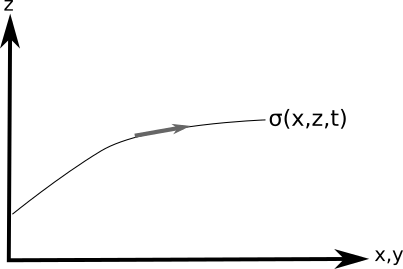
\includegraphics[width=0.4\textwidth]{figures/lecture13_exampleA.png}
	\caption{Schematic view of the steady and material $\sigma$-surface case, where the flow is along the surface. The grey vector shows the vector of the fluid particle velocity between time $t$ and $t+\delta t$.}
	\label{exA}
\end{figure}

\subsubsection*{Example B -- Non-steady and material $\sigma$-surface in $x$-direction} 


In this case, the material $\sigma$-surface ($\mathrm{D}\sigma/\mathrm{D}t = \dot{\sigma} = 0$) moves in time $\partial \sigma / \partial t \neq 0$. Therefore, the velocity vector becomes:
\begin{equation}
\boldsymbol{v} = \underbrace{u\bigg [\boldsymbol{\hat{x}} + \boldsymbol{\hat{z}}  \bigg (\frac{\partial z}{\partial x} \bigg )_\sigma \bigg]}_\text{motion along the surface}
	+ \underbrace{\bigg [ \bigg (\frac{\partial z}{\partial t}\bigg )_\sigma \bigg]\boldsymbol{\hat{z}}}_{\substack{\text{takes particle}\\\text{to the new $\sigma$-surface}}} ,
\end{equation}
as illustrated by the Figure~\ref{exB}.


\begin{figure}[h!]
	\centering
	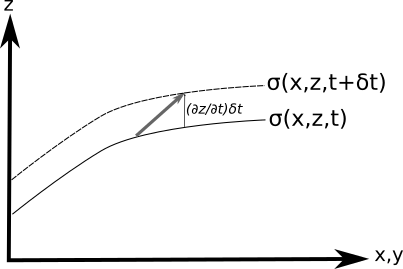
\includegraphics[width=0.4\textwidth]{figures/lecture13_exampleB.png} 
	\caption{Schematic view of the non-steady and material $\sigma$-surface case, where the fluid particle must move vertically relative to the static $\sigma$-surface. The grey vector shows the vector of the fluid particle velocity between time $t$ and $t+\delta t$.}
	\label{exB}
\end{figure}


\subsubsection*{Example C -- Non-steady and non-material $\sigma$-surface in $x$-direction} 

In this case, $\mathrm{D}\sigma/\mathrm{D}t = \dot{\sigma} \neq 0$ and $\partial \sigma/ \partial t \neq 0$. The third term in equation \eqref{vel}, including the dia-surface velocity ($w^{(\dot{\sigma})}$), cannot be neglected. $w^{(\dot{\sigma})}$ is the transport across the surface, which is not necessarily solely horizontal or vertical. Therefore, the velocity vector is:
\begin{equation}
\boldsymbol{v} = u\bigg [\boldsymbol{\hat{x}} + \boldsymbol{\hat{z}}  \bigg (\frac{\partial z}{\partial x} \bigg )_\sigma \bigg]
+ \bigg [ \bigg (\frac{\partial z}{\partial t}\bigg )_\sigma + \underbrace{w^{(\dot{\sigma})}}_{\substack{\text{dia-surface}\\\text{velocity}}} \bigg]\boldsymbol{\hat{z}} ,
\end{equation}
as illustrated by the Figure~\ref{exC}.

\begin{figure}[h!]
	\centering
	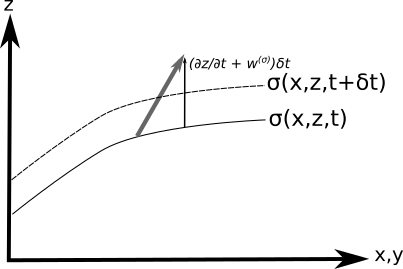
\includegraphics[width=0.4\textwidth]{figures/lecture13_exampleC.png}
	\caption{Schematic view of the non-steady and non-material $\sigma$-surface case, where the fluid particle must move vertically relative to the static $\sigma$-surface and cross the $\sigma$-surface. The grey vector shows the vector of the fluid particle velocity between time $t$ and $t+\delta t$, which departed from the $\sigma$-surface due to the nonzero dia-surface velocity component.}
	\label{exC}
\end{figure}

For more details, also read \citep[Chapter 18.3-18.6 in][]{Griffies2019}.